\chapter{Decay Widths of ICD-like Processes in the Asymptotic Limit}

Excited electronic states decaying in ICD or ETMD processes are an example
of resonance states. In the Fano-Feshbach theory of resonances they are
depicted as bound states embedded into and interacting with the
continuum \cite{Fano61,Feshbach58,Feshbach62}. Formally, the eigenstates
of the Hamiltonian in the vicinity of a resonance can be represented as a linear
superposition of the square integrable ``decaying state'' $\ket{\Phi}$ and
the continuum states $\ket{\chi_{\beta,\varepsilon}}$ satisfying ingoing
boundary conditions where $\varepsilon$ is the energy of the outgoing electron
and $\beta$ enumerates open decay channels. These states obey the following
normalization conditions

\begin{equation}
\braket{\Phi|\Phi}=1,\quad     
\braket{\chi_{\alpha,\varepsilon}|\chi_{\beta,\varepsilon^\prime}}=\delta_{\alpha\beta}
\delta(\varepsilon-\varepsilon^\prime),
\label{eq1}
\end{equation}
and one usually assumes that the continuum states prediagonalize the Hamiltonian $\hat{H}$
\begin{equation}
\braket{\chi_{\alpha,\varepsilon}|\hat{H}|\chi_{\beta,\varepsilon^\prime}}=\varepsilon\delta_{\alpha\beta}
\delta(\varepsilon -\varepsilon^\prime).
\label{eq2}
\end{equation}
We further assume the decaying and continuum states to be orthogonal
\begin{equation}
 \braket{\Phi|\chi_{\beta,\varepsilon}} = 0.
\end{equation}
The partial decay width $\Gamma_\beta$ in the lowest order of perturbation theory is given by \cite{Howat82}
\begin{equation}
\Gamma_\beta (E_\Phi) =2\pi\left |\braket{\chi_{\beta,\varepsilon}|\hat{H}-E_{\Phi}|\Phi}\right |^2,
\label{golden}
\end{equation}
where $E_{\Phi}=\braket{\Phi|\hat{H}|\Phi}$ is the resonance energy and
the energy of the final state is $\varepsilon = E_\Phi$. The total decay
width $\Gamma$ is obtained as the sum over all partial widths
$\Gamma = \sum\limits_{\beta} \Gamma_\beta$.

The expression in Eq.(\ref{golden}) represents a suitable starting point for
the {\it ab initio} computation of radiationless decay widths \cite{Howat82,Averbukh09_2}.
However, in the case of interatomic decay processes such as ICD or ETMD3,
simple analytic expressions can be derived for the case of large interatomic
distances between the monomers. For ICD such an expression was derived previously
in the nonrelativistic limit and was shown to be accurate for the interatomic
distances where the orbital overlap between the monomers is
negligible \cite{Averbukh04,Gokhberg10_1}. This formula is valid in the nonrelativistic
regime and becomes inadequate for systems exhibiting pronounced relativistic effects.
Therefore, we derive in the following analogous expressions for the case
when $\hat{H}$ is the many-electron Dirac-Coulomb Hamiltonian $\hat{H}_{DC}$ according
to
\begin{equation}
    \hat{H}_{DC}=\sum_{i=1}^N\left(c\vec{\alpha}_i\cdot\vec{p}_i + \beta_i m_ec^2 +
   \hat{V}_{\rm ext}(i){\bf{1}}_4\right) + \sum_{i<j}^N\frac{1}{r_{ij}}\, .
\end{equation}
Hereby $\vec{\alpha}_i$ and $\beta_i$ are the usual $4\times 4$ Dirac matrices
for particle $i$ in the standard notation.
In the electron-electron interaction term magnetic (Gaunt) contributions to
the Coulomb term and retardation effects are neglected. As can be seen in
Eq.(\ref{eq2}) already in the nonrelativistic case continuum functions not
normalizable in an $L^2$ sense appear in the positive energy range together with
discrete, normalizable bound states. As an additional difficulty coming along with
the use of $\hat{H}_{DC}$ one has to mention that, strictly speaking, there are no
normalizable many-electron eigenfunctions of $\hat{H}_{DC}$
\cite{brown51, sucher80, pestka2006, bylicki2008} requiring the extra condition
that the negative energy eigenstates be not accessible. We therefore work with a
DC Hamiltonian that is projected onto the space of the positive energy states
allowing for a construction of a normalizable many-electron basis describing
bound states together with continuum states lying in the positive energy range.
For actual implementations, the operators are generally used in their second-quantized
form. As a consequence of the projection of $\hat{H}_{DC}$, the corresponding
creation and annihilation operators act in the positive energy space exclusively
(no pair formalism, see e.g. \cite{grant88}) and refer to occupied and virtual
one-particle states from which the many-particle wave functions are built.

Now we turn our attention to the system under investigation.
Let $\mathbf{S}_1$ and $\mathbf{S}_2$ denote two subsystems participating in the
interatomic or intermolecular decay which are located at a distance $R$ from each
other. We assume that the initial inner-valence vacancy resides on $\mathbf{S}_1$.
In the decay, an outer-valence electron of $\mathbf{S}_1$ fills the inner-valence
vacany, while an outer-valence electron of $\mathbf{S}_2$ is being ionized in the
process. The chosen general partitioning is suitable for the description of ICD
and ETMD3 processes. In the latter case the two monomers participating in the
charge transfer are combined to one subsystem and the third monomer which is ionized
forms the second subsystem. 

The $(N-1)$-electron Hamiltonian $\hat{H}_{DC}$ can be written as
\begin{equation}\label{sepHDC}
 \hat{H}_{DC} = \hat{H}_{S_1} + \hat{H}_{S_2} + \hat{H}_{S_1,S_2},
\end{equation}
where $\hat{H}_{S_k} = \sum\limits_{i\in S_k}^{N_{S_k}} \hat{h}_{DC}(i)
                       + \sum\limits_{i>j; i,j\in S_k}^{N_{S_k}} \frac{1}{r_{ij}}$
denotes the Hamilton operator of the electrons residing on subsystem
$\mathbf{S}_k$ ($k=1,2$) consisting of the corresponding one-electron part and
the Coulomb interaction between electrons localized within the
subsystem $\mathbf{S}_k$ and
$\hat{H}_{S_1,S_2} = \hat{V}_{S_1,S_2} = \sum\limits_{i\in S_1, j\in S_2}^N \frac{1}{r_{ij}}$
describes the Coulomb interaction between electrons located on different subsystems.
At large distances between the monomers the decaying and continuum states can be
approximated by the product forms 
\begin{align}\label{sepWF}
 \ket{\Phi}                       &= \ket{\phi_{iv}^{(S_1)}}   \ket{\phi_{0}^{(S_2)}} \nonumber\\
 \ket{\chi_{\beta,\varepsilon}} &= \ket{\phi_{ov_1}^{(S_1)}} \ket{\chi_{ov_2,\varepsilon}^{(S_2)}}.
\end{align}
Here $\ket{\phi_{iv}^{(S_1)}}$ and $\ket{\phi_{ov_1}^{(S_1)}}$ are othogonal
eigenstates of the Hamilton operator $\hat{H}_{S_1}$ of subsystem $\mathbf{S}_1$
describing the inner-valence ($iv$) and outer-valence ($ov_1$) ionized states of
$\mathbf{S}_1$. The states $\ket{\phi_{0}^{(S_2)}}$ and $\ket{\chi_{ov_2,\varepsilon}^{(S_2)}}$
are the ground state of $\mathbf{S}_2$ and a scattering state
$\ket{\chi_{ov_2,\varepsilon}^{(S_2)}}$ corresponding to the outer-valence vacancy ($ov_2$)
of $\mathbf{S}_2$ and a free electron of energy $\varepsilon$. The bound and the continuum
state of $\mathbf{S}_2$ in Eq. (\ref{sepWF}) are, therefore, orthogonal by construction.

Inserting the Dirac-Coulomb Hamiltionian Eq. (\ref{sepHDC}) and the wavefunctions
in Eq. (\ref{sepWF}) into the expression for the decay rate in Eq. (\ref{golden})
and using the orthogonality relations, we arrive at the following expression for
the partial decay width
\begin{equation}\label{relgolden}
 \Gamma_\beta=2\pi\left |\braket{\chi_{\beta,\varepsilon}|\hat{V}_{S_1,S_2}|\Phi}\right |^2,
\end{equation}
where $\beta$ denotes the combination of electrons involved in the corresponding pathways.

This expression was first obtained by Wentzel \cite{Wentzel27,Aagren92} for the Auger
decay widths. Its applicability is limited to processes where the coupling of the
discrete and continuum states is weak and which can be treated as two-step processes,
which means, that the electronic decay is independent of the primary ionization process.
Both requirements are fulfilled for the ICD and ETMD processes discussed in this paper.

\begin{figure}[ht]
\centering
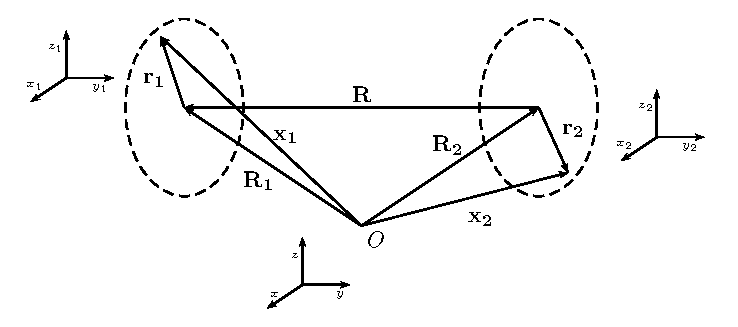
\includegraphics[scale=1.0]{pics/taylor_pspic.eps}
%\input{taylor_pspic}
\caption{The total system is split into subsystems $\mathbf{S_1}$ and $\mathbf{S_2}$.
The $\mathbf{R}_i$ ($i=1,2$)  point to the corresponding  centers of mass (COMs)
with respect to an arbitrary origin $O$. The $\mathbf{x}_i$ as well as the $\mathbf{r}_i$
describe the electron coordinates once with respect to $O$ and once with respect to the COMs.}
\label{taylor_pspic}
\end{figure}

In order to arrive at working expressions we expand the
Coulomb interaction $\hat{V}_{S_1,S_2}$ in powers of $\frac 1R$ obtaining the
asymptotic expansion \cite{santra2002}:

\begin{align}\label{taylor_multi}
\frac{1}{\left| \mathbf{x}_1-\mathbf{x}_2 \right|} = \frac 1R - \frac{\mathbf{\hat{u}}_R \cdot (\mathbf{r}_1-\mathbf{r}_2)}{R^2}
+ \frac{3(\mathbf{\hat{u}}_R \cdot (\mathbf{r}_1-\mathbf{r}_2))^2 - (\mathbf{r}_1-\mathbf{r}_2)^2}{2R^3} + \mathcal{O} \left( \frac 1{R^4} \right)
\end{align}
where $R=|\mathbf{R}| = |\mathbf{R}_1-\mathbf{R}_2|$ is the distance between the COMs
(see Fig.\ref{taylor_pspic}) and $\mathbf{\hat{u}}_R =  \mathbf{R}/|\mathbf{R}|$ is
the unit vector along $\mathbf{R}$. Each of the subsystems has its own coordinate system
residing in the respective center of mass. Such an expansion converges uniformly
if $|\mathbf{r_i}|<R/2$, corresponding to the absence of overlap of electron
densities localized on different subsystems \cite{Ahlrichs76}. We truncate
the series in Eq. (\ref{taylor_multi}) after the third
term and focus on dipole transitions alone. Inserting it into Eq.(\ref{relgolden}) yields
\begin{align}\label{taylor_in}
\Braket{\chi_{\beta,\varepsilon}|\hat{V}_{S_1,S_2}|\Phi} 
          =&  -\frac{3}{R^3} \Braket{\phi_{ov_1}^{(S_1)}|\sum\limits_i \mathbf{r}_1^{(i)}\cdot\mathbf{\hat{u}}_R|\phi_{iv}^{(S_1)}}
           \cdot \Braket{\phi_{0}^{(S_2)}|\sum\limits_j \mathbf{r}_2^{(j)}\cdot\mathbf{\hat{u}}_R|\chi_{ov_2,\varepsilon}^{(S_2)}}
           \nonumber\\
          &+\frac{1}{R^3} \Braket{\phi_{ov_1}^{(S_1)}|\sum\limits_i \mathbf{r}_1^{(i)}|\phi_{iv}^{(S_1)}} \cdot
            \Braket{\phi_{0}^{(S_2)}|\sum\limits_j \mathbf{r}_2^{(j)}|\chi_{ov_2,\varepsilon}^{(S_2)}}
\end{align}
where we made use of the fact that the matrix elements over the first two terms
in the expansion (\ref{taylor_multi}) vanish due to orthogonality of the
decaying and final continuum states. For rewriting Eq.(\ref{taylor_in}) in
spherical coordinates it is convenient to orient $\mathbf{R}$ along the $z_2$ axis leading to
\begin{align}\label{last_matrixelement}
 \braket{\chi_{\beta,\varepsilon}|\hat{V}_{S_1,S_2}|\Phi} 
= \frac{1}{R^3} \sum\limits_{m=0,\pm 1} B_m \braket{\phi_{ov_1}^{(S_1)}|{D}_{1m}|\phi_{iv}^{(S_1)}}  \braket{\phi_{0}^{(S_2)}|{D}_{2m}|\chi_{ov_2,\varepsilon}^{(S_2)}} ,
\end{align}
where $B_0=-2$, $B_{\pm 1}=1$ and $D_{im} = \sum\limits_{i} r_{im}$ ($i=1,2$) are
the dipole operators acting on the electron coordinates of the
subsystems $\mathbf{S_1}$ and $\mathbf{S_2}$, respectively (see \cite{9} for
further details). The general expression for the decay width $\Gamma_\beta$
referring to the decay process then reads as

\begin{align}
\label{sum_squares}
\Gamma_\beta
=  \frac{2\pi}{R^6}\sum\limits_{m=0,\pm 1}B_m^2 \left|
\braket{\phi_{ov_1}^{(S_1)}|{D}_{1m}|\phi_{iv}^{(S_1)}}\right|^2
\left|\braket{\phi_{0}^{(S_2)}|{D}_{2m}|\chi_{ov_2,\varepsilon}^{(S_2)}}\right|^2
\end{align}
and serves as the starting equation for the special cases of ICD and ETMD3
as discussed in the following subsections.

\section{Interatomic Coulombic Decay}
\label{subs_icd}

\begin{figure}[ht]
\centering
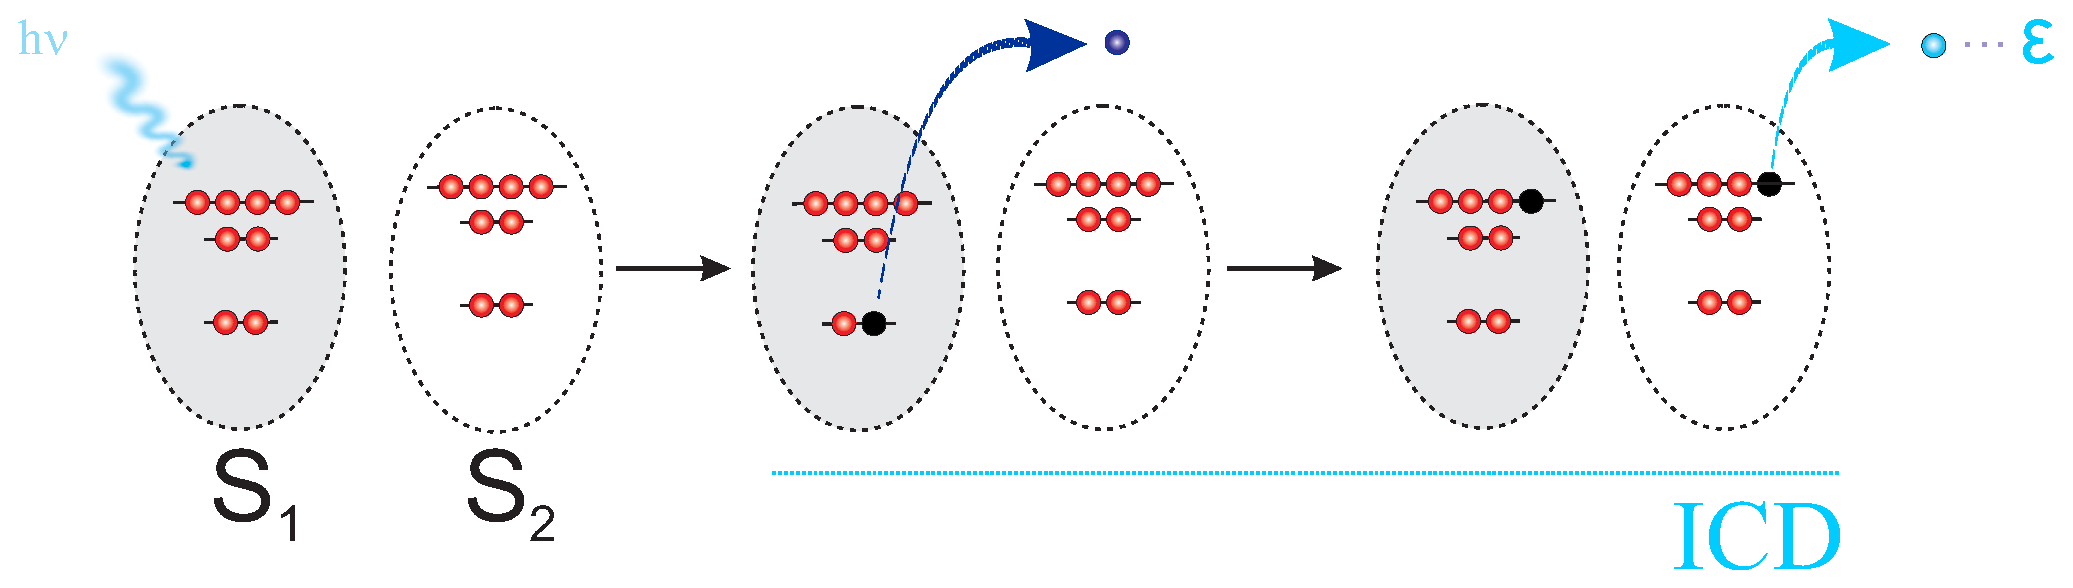
\includegraphics[scale=0.30]{pics/ICD_subsystems.eps}
\caption{ICD process in subsystems $\mathbf{S_1}$ and $\mathbf{S_2}$. After
         creating an inner valence vacancy in $\mathbf{S_1}$  the hole is filled
         by an outer-valance electron of $\mathbf{S_1}$. The excess energy is
         transferred to $\mathbf{S_2}$ and is used to remove an outer-valence
         electron (ICD electron).}
\label{fancy_ICD}
\end{figure}

In the ICD process the inner valence vacancy is filled with an electron
of the same atom or molecule. The excess energy is transferred to the secon
subunit and is used to ionize it (see Fig. \ref{fancy_ICD}). In rare gas
clusters the corresponding subunits are atoms leading to the partition
$\mathbf{S_1}$ as atom $A$ and $\mathbf{S_2}$ as atom $B$. In atoms,
the total angular momentum quantum number $J$ and its projection $M$ are
good quantum numbers. As an ansatz for the initial and final state wave
functions under the assumption of no interaction, the product of individual
atomic configuration state functions is taken:
\begin{equation}\label{wf_ansatz}
\ket{\Phi} =\ket{E_A\, J_A\, M_A}\ket{E_B\, J_B\, M_B}
\quad\mbox{and}\quad
\ket{\chi_{\beta,\varepsilon}} = \ket{E'_A\, J'_A\, M'_A}\ket{E'_B\,  J'_B\, M_B'}\, .
\end{equation}
In this expression the initial and final states are characterized by the
energies of the atoms $E_A$, $E_B$ and $E_A'$, $E_B'$, the corresponding
total angular momenta of the atoms are denoted as $J_A$, $J_B$ and
$J_A'$, $J_B'$ and their projections on the $z$-axis as $M_A$, $M_B$ and
$M_A'$, $M_B'$, respectively. At the beginning of the process atom $B$ is
assumed to be in its closed shell ground state $\ket{\Phi_0^{(B)}}$ with
$J_B=M_B=0$. Inserting Eqs. (\ref{wf_ansatz}) into (\ref{sum_squares})
we obtain

\begin{align}
\label{Gamma_ICD_allsum}
\Gamma_\beta =& \frac{2\pi}{R^6} \sum\limits_{m} \, B_{m}^2 \, \left| \braket{E'_A\, J'_A\, M'_A | \hat{D}^{(A)}_{m} | E\, J_A\, M_A}\right|^2 \nonumber\\
        & \times\, \left| \braket{\Phi_0^{(B)} | \hat{D}^{(B)}_{m} | E'_B\, J'_B\, M_B'}^* \right|^2\, \delta (E-E')
\end{align}

At large distances the energies of the decaying and final state can be
assumed to be the sum of the energies of the two subsystems
$A$ and $B$: $E=E_A+E_B$, $E'=E_A'+E_B'$. The resonance condition $E=E'$
can therefore be expressed through the energy matching of virtual photons
emitted in the transition on atom $A$, $\omega_A=E_A-E'_A$, and absorbed
by atom $B$, $\omega_B=E_B'-E_B$, i.e. $\omega_A=\omega_B=\omega_{vp}$.
We can use the conservation of the projection of the angular momentum on
the $z$-axis $M_A=M_A'+M_B'$ to further simplify the expression in
Eq. (\ref{Gamma_ICD_allsum}). By setting $m=-M_B'$ and using the
Wigner-Eckart theorem \cite{EdmondsAngular} we arrive at

\begin{align}\label{reltheolifetime}
 \Gamma_\beta =& \frac{2\pi}{R^6} \sum\limits_{M_A'} \, B_{M_A'-M_A}^2 \, \left| \left(
\begin{array}{ccc}
J_A'  & 1        & J_A\\
-M_A' & M_A'-M_A & M_A
\end{array}\right)
 \braket{E'_A\, J'_A || \hat{D}^{(A)} || E\, J_A}\right|^2 \nonumber\\
        & \times\, \frac 13  \left| \braket{\Phi_0^{(B)} || \hat{D}^{(B)} || E'_B\, J'_B} \right|^2,
\end{align}
where each decay channel $\beta$ is characterized by $E_A'$, $J_A'$, $E_B'$
and $J_B'$.

To find numerical values of $\Gamma_\beta$, the necessary dipole transition
moments of the isolated atoms in Eq. (\ref{reltheolifetime}) can either
be computed directly or obtained from experimentally accessible quantities.
At first we use the fact that the square of the reduced matrix element of
atom $A$, the so-called line strength, is proportional to the state-to-state
transition probability $W_{J_A,J_A'}$, which is in turn the inverse of the
radiative lifetime $\tau$ of the initial state \cite{Sobelman72}:

\begin{equation}
\label{sysa_emission}
  \left| \braket{E'_A\, J'_A || \hat{D}^{(A)} || E\, J_A} \right|^2 = (2J_A +1)\, \frac{3c^3}{4\omega_{vp}^3}\, W_{J_A,J_A'} .
\end{equation}
Second, the square of the reduced matrix element of atom $B$ is related
to its partial  photoionization cross section $\sigma^{(B)}(\omega_{vp})$
which depends on the energy atom $B$ is exposed to \cite{Sobelman72}:

\begin{equation}\label{sysb_absorption}
  \left| \braket{\Phi_0^{(B)} || \hat{D}^{(B)} || E'_{B}\, J'_{B}} \right|^2
   = \frac{3c\,\sigma^{(B)}(\omega_{vp})}{4\pi^2\omega_{vp}} .
\end{equation}
After insertion of Eq.(\ref{sysa_emission}) and (\ref{sysb_absorption})
into (\ref{reltheolifetime}) we arrive at a working expression for the
partial decay width according to

\begin{align}\label{reltheolifetime_exp}
 \Gamma_\beta =& \frac{2\pi}{R^6} \sum\limits_{M_A'} \, B_{M_A'-M_A}^2 \, \left| \left(
\begin{array}{ccc}
J_A'  & 1        & J_A\\
-M_A' & M_A'-M_A & M_A
\end{array}\right) \right|^2
 (2J_A+1)\frac{3c^4 \sigma^{(B)}(\omega_{vp})}{16\pi^2\omega_{vp}^4\tau_A} .
\end{align}
As could be expected from the nonrelativistic formula, the relativistic
expression also shows an $R^{-6}$-behaviour for the energy transfer
corresponding to the interaction of two dipoles.
Setting atomic parameters to their non-relativistic values and summing
over all partial decay widths 
$\Gamma=\sum\limits_\beta \Gamma_\beta$ produces the known
non-relativistic result for the total decay width \cite{Averbukh04,Gokhberg10_1}.

One of our major goals is the inclusion of relativistic effects in the
computation of the decay widths which is achieved by using $J/M_J$ adapted
initial and final state wave functions. As a result, we observe more
energetically distinguishable decay pathways leading to a different energy
distribution of the emitted ICD electrons compared to the nonrelativistic
description. Moreover, if ICD takes place close to its threshold, the number
of open channels might differ in the two cases resulting in different total
ICD rates.

%$$$$$$$$$$$$$$$$$$$$$$$$$$$$$$$$$$$$$$$$$$$$$$$$$$$$$$$$$$$$$$$$$$$$$$$$$$$

\section{Electron Transfer Mediated Decay}
\label{subs_etmd}

\begin{figure}[ht]
\centering
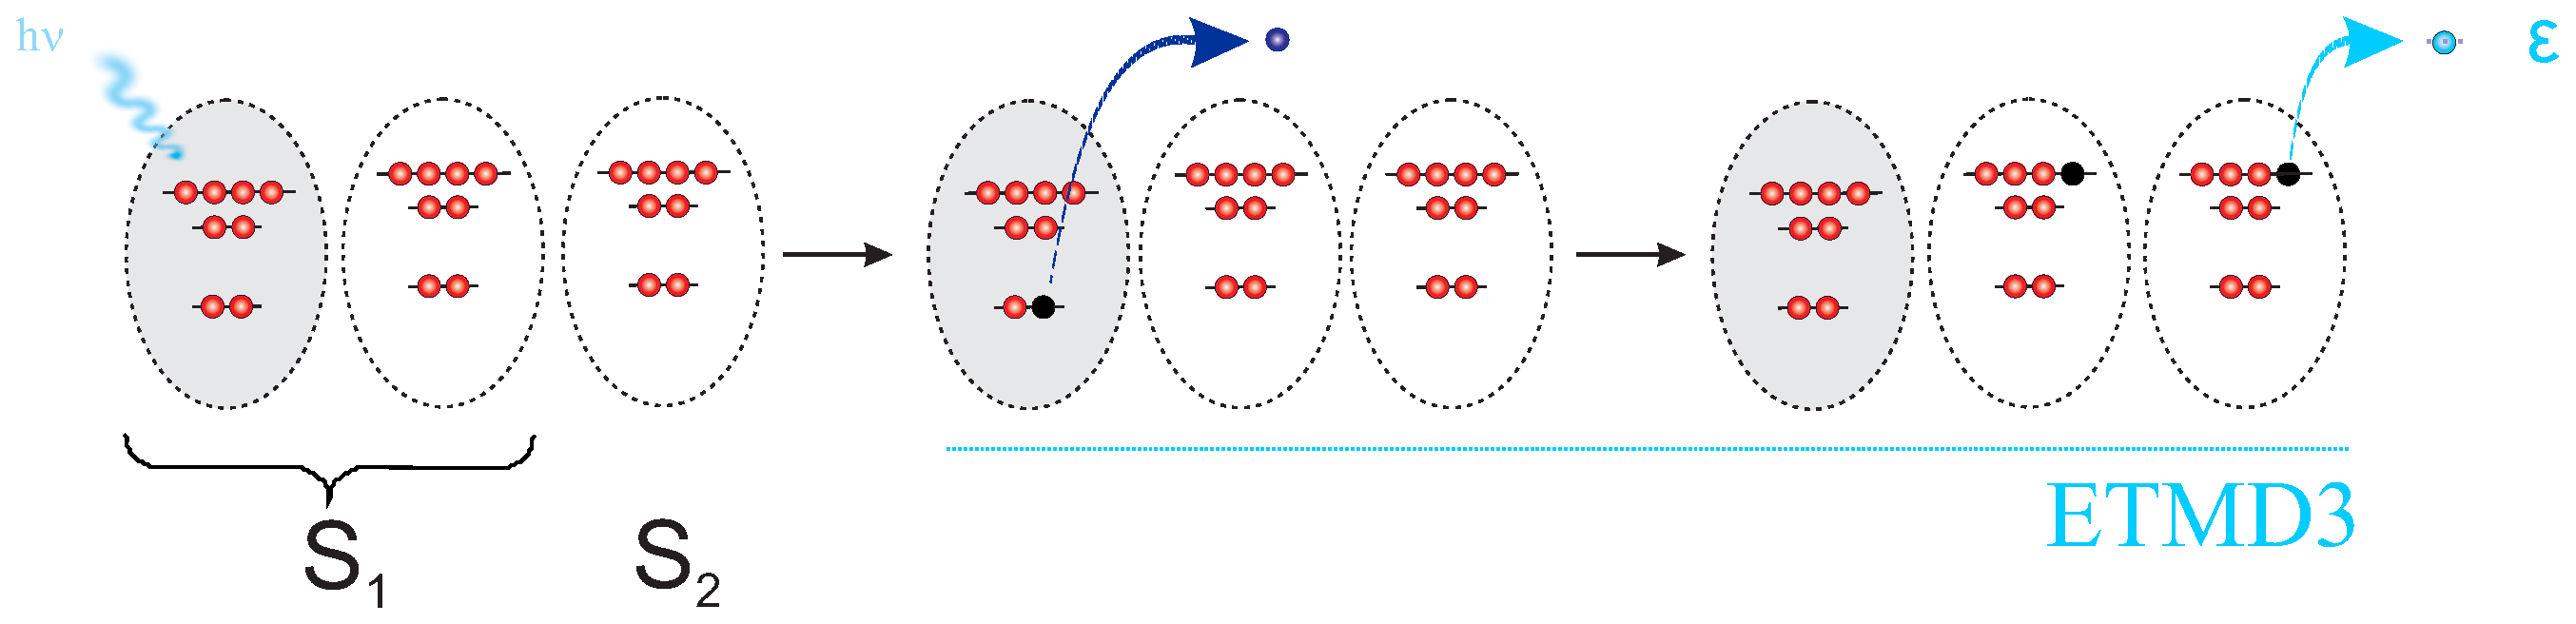
\includegraphics[scale=0.30]{pics/ETMD_subsystems.eps}
\caption{ETMD3 process in subsystems $\mathbf{S_1}$ and $\mathbf{S_2}$ where
         the two atoms A and B participate in the electron transfer and are
         combined to $\mathbf{S_1}$. After inner valence ionization of A,
         the vacancy is filled by an electron from B in $\mathbf{S_1}$.
         The energy is transferred to C ($\mathbf{S_2}$) which is ionized
         and hereby emits the ETMD electron.}
\label{fancy_ETMD}
\end{figure}

In the ETMD3 process (see Fig. \ref{fancy_ETMD}) three atoms are involved
which we denote by $A$, $B$ and $C$. The two subsystems in this case are
$AB$ ($\mathbf{S}_1$) and $C$ ($\mathbf{S}_2$). The initial inner valence
hole is assumed to be located on atom $A$. The electron is transferred
from atom $B$ to atom $A$, while the excess energy is transferred from
$\mathbf{S_1}$ to atom $C$ and used to ionize it. For a convenient
geometric description of the triatomic system undergoing the ETMD3 process
we use Jacobi coordinates as shown in Fig.\ref{etmd_geom_pspic}. All
properties of the $AB$ comprising subsystem $\mathbf{S_1}$ are described in
its local $(\tilde{x}_1, \tilde{y}_1,  \tilde{z}_1)$ coordinate system which
is later backtransformed.

Analog to eq. (\ref{last_matrixelement}) we arrive at

\begin{align}\label{last_matrixelement_etmd}
 \braket{\chi_{\beta,\varepsilon}|\hat{V}_{S_1,S_2}|\Phi} 
=& \frac{1}{R^3} \sum\limits_{ov_1,ov_2,\varepsilon}  \left[
  \braket{\phi_{ov_1}^{(S_1)}|  \begin{pmatrix}
         -\frac{1}{\sqrt{2}}(\tilde{x}_1\cos\alpha- \tilde{z}_1\sin\alpha +i\tilde{y}_1)\\
         \frac{1}{\sqrt{2}}(\tilde{x}_1\cos\alpha- \tilde{z}_1\sin\alpha -i\tilde{y}_1)\\
         -2 (\tilde{x}_1\sin\alpha + \tilde{z}_1\cos\alpha )\\
         \end{pmatrix} |\phi_{iv}^{(S_1)}} \right. \nonumber \\
  & \cdot \left. \braket{\phi_{0}^{(S_2)}| \begin{pmatrix}
                            r_{2+}\\
                            r_{2-}\\
                            r_0\\
                            \end{pmatrix} |\chi_{ov_2,\varepsilon}^{(S_2)}} \right] .
\end{align}

\begin{figure}[ht]
\centering
%\input{coord_etmd_pspic}
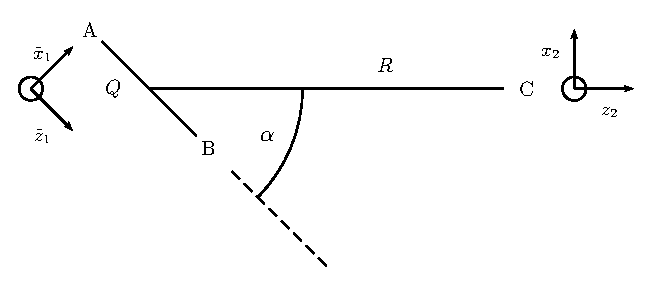
\includegraphics[scale=1.00]{pics/coord_etmd_pspic.eps}
\caption{Jacobi coordinates used for the geometric description of the trimer.
        $Q$ is the distance between $A$ and $B$, $R$ the distance from the
        center of mass of $AB$ to $C$ and $\alpha$ the angle between the
        lines represented by $Q$ and $R$.}
\label{etmd_geom_pspic}
\end{figure}

We define the initial state of ETMD as
$\ket{\Phi} = \ket{E_{AB}\,  M_{AB}}\ket{\Phi_0^{(C)}}$ and the final state
as $\ket{\chi_{\beta,\varepsilon}} = \ket{E_{AB}'\, M_{AB}'}\ket{E_C'\,   J_C'\, M_C'}$,
where $E_{AB}$ and $E_{AB}'$, $E_C'$ are the energies of the corresponding
initial and final states of the subsystems. Since the subsystem $AB$ is of
linear symmetry the total angular momentum $J_{AB}$ is no longer a good
quantum number but the projections $M_{AB}$, $M_{AB}'$ still are and serve
for the characterization of $AB$. $J_C'$ is the total angular momentum of $C$
in its final state and $\ket{\Phi_0^{(C)}}$ is the closed shell ground
state of atom $C$ in its initial state. Using Eq. (\ref{sum_squares})
and expressing the electron dipole
moment $\vec{D}_1$ of $\mathbf{S}_1$ in the coordinates
($\tilde{x}_1,\tilde{y}_1,\tilde{z}_1$) we arrive at an intermediate equation
for $\Gamma_\beta$ as

\begin{align} \label{reltheolifetimeetmd}
 \Gamma_\beta =& \frac{2\pi}{R^6} \sum\limits_{M_{AB}'} \left[ 2\left( \left|
                 \braket{M_{AB}'| \tilde{D}_x |M_{AB}} \right|^2 (1+  \cos^2\alpha)
                 + \left|\braket{M_{AB}'| \tilde{D}_z |M_{AB}}\right|^2 \sin^2\alpha \right) \right. \nonumber \\
           & \quad\left.+ 4 \left( \left|\braket{M_{AB}'| \tilde{D}_x |M_{AB}}
             \right|^2\sin^2\alpha
             + \left|\braket{M_{AB}'| \tilde{D}_z |M_{AB}}\right|^2\cos^2\alpha \right)  \right] \nonumber\\ 
           & \times\, \frac 13  \left| \braket{\Phi_0^{(C)} || \hat{D}^{(C)} ||J'_C} \right|^2
         ,
\end{align}
where each decay channel $\beta$ is characterized by its own $E_{AB}'$, $E_C'$
and $J_C'$. The reduced matrix elements of atom $C$ can again be expressed in
terms of its ionization cross section
\begin{equation}\label{mecross}
  \left| \braket{\Phi_0^{(C)} || \hat{D}^{(C)} || E'_{C}\, J'_{C}} \right|^2
   = \frac{3c\,\sigma^{(C)}(\omega_{vp})}{4\pi^2\omega_{vp}} 
\end{equation}
and the transition dipole moments of $AB$ can be conveniently computed
using quantum chemical program packages.
Finally we arrive at the following working equation for the decay
width according to
\begin{align} \label{reltheolifetimeetmd_exp}
 \Gamma_\beta =& \frac{2\pi}{R^6} \sum\limits_{M_{AB}'} \left[ 2\left( \left| \braket{M_{AB}'| \tilde{D}_x |M_{AB}} \right|^2 (1+ \cos^2\alpha) + \left|\braket{M_{AB}'| \tilde{D}_z |M_{AB}}\right|^2 \sin^2\alpha \right) \right. \nonumber \\
           & \quad\left.+ 4 \left( \left|\braket{M_{AB}'| \tilde{D}_x |M_{AB}}\right|^2\sin^2\alpha + \left|\braket{M_{AB}'| \tilde{D}_z |M_{AB}}\right|^2\cos^2\alpha \right)  \right] \nonumber \\ 
           & \times\, \frac{c\sigma^{(C)}(\omega_{vp})}{4\pi^2 \omega_{vp}}
           \delta (\omega_{AB}-\omega_C) .
\end{align}

The corresponding nonrelativistic expression for the ETMD decay width is
obtained by using $L$ and $S$ instead of the total angular momentum $J$ for
each electronic state together with the nonrelativistic virtual photon
energy and the corresponding photoionization cross section. Analogously to
the ICD we observe the $R^{-6}$ behaviour of the energy transfer.
Additionally, an $e^{-\alpha Q}$ dependence is hidden in the transition
dipole moments due to the charge transfer occurring in the ETMD process.


